%% 
%% Copyright 2007-2025 Elsevier Ltd
%% 
%% This file is part of the 'Elsarticle Bundle'.
%% ---------------------------------------------
%% 
%% It may be distributed under the conditions of the LaTeX Project Public
%% License, either version 1.3 of this license or (at your option) any
%% later version.  The latest version of this license is in
%%    http://www.latex-project.org/lppl.txt
%% and version 1.3 or later is part of all distributions of LaTeX
%% version 1999/12/01 or later.
%% 
%% The list of all files belonging to the 'Elsarticle Bundle' is
%% given in the file `manifest.txt'.
%% 
%% Template article for Elsevier's document class `elsarticle'
%% with numbered style bibliographic references
%% SP 2008/03/01
%% $Id: elsarticle-template-num.tex 272 2025-01-09 17:36:26Z rishi $
%%
\documentclass[preprint,12pt]{elsarticle}

%% Use the option review to obtain double line spacing
%% \documentclass[authoryear,preprint,review,12pt]{elsarticle}

%% Use the options 1p,twocolumn; 3p; 3p,twocolumn; 5p; or 5p,twocolumn
%% for a journal layout:
%% \documentclass[final,1p,times]{elsarticle}
%% \documentclass[final,1p,times,twocolumn]{elsarticle}
%% \documentclass[final,3p,times]{elsarticle}
%% \documentclass[final,3p,times,twocolumn]{elsarticle}
%% \documentclass[final,5p,times]{elsarticle}
%% \documentclass[final,5p,times,twocolumn]{elsarticle}

%% For including figures, graphicx.sty has been loaded in
%% elsarticle.cls. If you prefer to use the old commands
%% please give \usepackage{epsfig}

%% The amssymb package provides various useful mathematical symbols
\usepackage{amssymb}
%% The amsmath package provides various useful equation environments.
\usepackage{amsmath}
%% The amsthm package provides extended theorem environments
%% \usepackage{amsthm}
\usepackage{array}
\usepackage{tabularx}
\usepackage{booktabs}
\usepackage{algorithm}
\usepackage{algorithmic}
\usepackage{soul}   % for \hl highlighting
\usepackage[normalem]{ulem} % for \sout strikethrough
\usepackage{xcolor}
% Define commands for marked version
\newcommand{\added}[1]{\hl{#1}}
\newcommand{\deleted}[1]{\textcolor{red}{\sout{#1}}}
\newcommand{\replaced}[2]{\hl{#1} \textcolor{red}{\sout{#2}}}\usepackage[markup=highlight,highlightcolor=yellow]{changes}
%% For clean version with changes accepted uncomment in the next 3 lines:
%%\renewcommand{\added}[1]{#1}
%%\renewcommand{\deleted}[1]{}
%%\renewcommand{\replaced}[2]{#1}

\journal{Journal of Theoretical Biology}

\begin{document}

\begin{frontmatter}

%% Title, authors and addresses

%% use the tnoteref command within \title for footnotes;
%% use the tnotetext command for theassociated footnote;
%% use the fnref command within \author or \affiliation for footnotes;
%% use the fntext command for theassociated footnote;
%% use the corref command within \author for corresponding author footnotes;
%% use the cortext command for theassociated footnote;
%% use the ead command for the email address,
%% and the form \ead[url] for the home page:
%% \title{Title\tnoteref{label1}}
%% \tnotetext[label1]{}
%% \author{Name\corref{cor1}\fnref{label2}}
%% \ead{email address}
%% \ead[url]{home page}
%% \fntext[label2]{}
%% \cortext[cor1]{}
%% \affiliation{organization={},
%%             addressline={},
%%             city={},
%%             postcode={},
%%             state={},
%%             country={}}
%% \fntext[label3]{}

\title{Stability-Driven Assembly Theory}

%% use optional labels to link authors explicitly to addresses:
%% \author[label1,label2]{}
%% \affiliation[label1]{organization={},
%%             addressline={},
%%             city={},
%%             postcode={},
%%             state={},
%%             country={}}
%%
%% \affiliation[label2]{organization={},
%%             addressline={},
%%             city={},
%%             postcode={},
%%             state={},
%%             country={}}

\author{Dan Adler} %% Author name

%% Author affiliation
\affiliation{email={dan@danadler.com}}

%% Abstract
\begin{abstract}
The emergence of complexity and information remains a fundamental question in all scientific disciplines. This paper introduces Stability-Driven Assembly (SDA) systems, a theoretical framework that models pattern evolution through probabilistic interactions governed by differential stability. Our computational experiments demonstrate that stability differences alone can generate selection pressure, driving systems toward lower-entropy states characterized by dominant stable patterns, without requiring explicit replication mechanisms. Through controlled intervention experiments, we establish a causal relationship \added{within the model} between stability constraints and system evolution, showing how stability functions as a control parameter shaping the evolutionary landscape. The SDA framework reveals the interplay between bottom-up assembly processes and top-down selective pressures, where emergent stable patterns recursively influence future interactions. Dynamic network visualization further illuminates how stability-driven selection operates on all scales. These findings \added{may provide the foundation for} \deleted{provide} a mechanistic explanation \replaced{of}{for} how complexity and information can emerge in abiotic systems\deleted{, with implications for understanding
prebiotic chemical evolution and the transition from inanimate to
living matter.}\added{. Looking ahead, we suggest that SDA could provide a useful lens for connecting stochastic dynamical systems with prebiotic chemistry, and for exploring hypotheses about how stability-driven dynamics might precede the emergence of autocatalysis, replication, and Darwinian evolution.}

\end{abstract}



%%Graphical abstract
\begin{graphicalabstract}
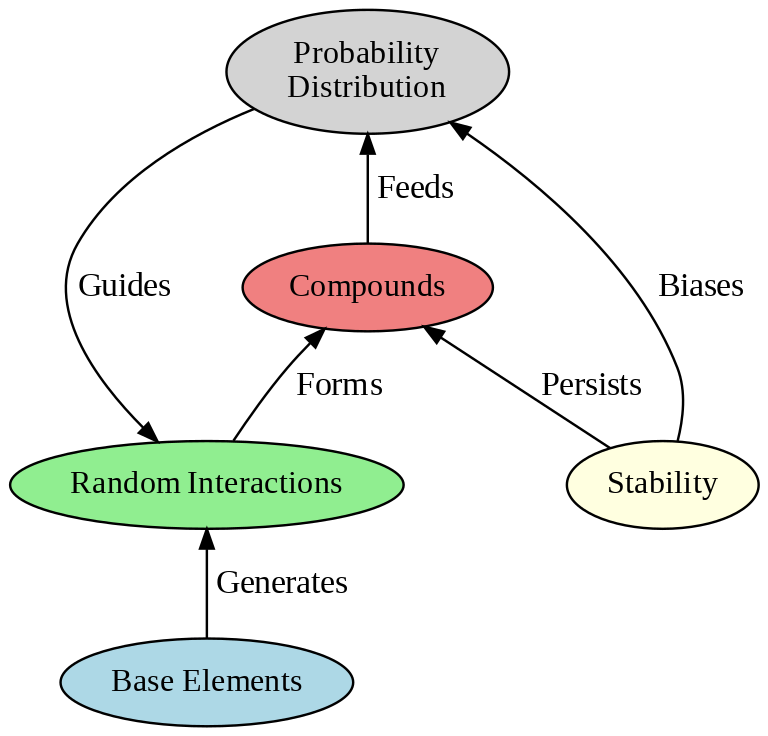
\includegraphics[width=1\textwidth]{figure_10}
\end{graphicalabstract}

%%Research highlights
\begin{highlights}
\item Establishes Stability-Driven Assembly (SDA) systems as a mathematical framework for modeling selection in abiotic systems.
\item Demonstrates through controlled intervention experiments the causal relationship between stability constraints and system evolution.
\item Proves that differential pattern persistence alone can generate evolutionary dynamics without explicit replication mechanisms.
\item Visualizes stability-driven selection through dynamic network representations and token flow analysis.
\item Provides a unifying framework for understanding pattern formation across chemical, physical, and information-processing systems.
\end{highlights}

%% Keywords
\begin{keyword}
Stability-driven selection; Abiotic evolution; Pattern formation; Emergent complexity; Entropy reduction; Evolutionary dynamics; Chemical evolution
\end{keyword}

 %% keywords here, in the form: keyword \sep keyword

%% PACS codes here, in the form: \PACS code \sep code

%% MSC codes here, in the form: \MSC code \sep code
%% or \MSC[2008] code \sep code (2000 is the default)

\end{frontmatter}

% The order of the section titles is different for some journals. Please refer to the "Instructions for Authors” on the journal homepage.

\section{Introduction}

"\textit{Selection for longevity becomes inseparable from selection for propagation. What persists has, by definition, a greater opportunity to propagate its structure.}" This observation by Stuart Kauffman \cite{kauffman1995home} identifies a fundamental principle that may bridge the gap between inanimate physical processes and biological evolution. Although the mechanisms of biological evolution through natural selection are well established \cite{fisher1930genetical}, the emergence of selection itself - prior to true replication - remains enigmatic.

In inanimate physical systems, patterns persist according to their stability under prevailing conditions. A carbon lattice in diamond form persists longer than graphite under high pressure; certain molecular configurations outlast others in various chemical environments \cite{davies2006goldilocks}. This differential persistence creates an implicit selection mechanism: stable configurations naturally become more prevalent over time simply by outlasting less stable alternatives. This fundamental principle of stability-driven selection may have preceded and enabled the emergence of biological selection \cite{hordijk2012autocatalytic, nghe2015prebiotic}.

The study of such selection mechanisms spans multiple scientific disciplines. Algorithmic complexity \cite{kolmogorov1965complexity, chaitin1977algorithmic, solomonoff1964formal} and Shannon's information theory \cite{shannon1948mathematical} provide tools to quantify patterns and information, but do not explain how information emerges from physical systems. Constructor theory \cite{deutsch2013constructor} reframes physical laws in terms of possible transformations, while Assembly Theory (AT) \cite{walker2023nature} quantifies complexity through the minimal steps needed to construct an object, but provides a retrospective rather than dynamic model of selection in real time.

The transition from inanimate systems to living systems represents one of the most profound questions of science \cite{schrodinger1944life, pross2016life}. Several theoretical frameworks have attempted to explain the emergence of complex, information-rich systems from simpler components. Particularly relevant to stability-driven selection are autocatalytic sets, developed by Kauffman \cite{kauffman1986autocatalytic} and further explored by Hordijk and Filisetti \cite{hordijk2011required}, which examine how networks of molecules can collectively catalyze each other's production. Similarly, Fontana's Artificial Chemistry (AlChemy) \cite{fontana1991algorithmic} uses lambda calculus to model chemical reactions and explores how self-maintaining networks of interacting molecules emerge. The preferential attachment network model introduced by Barabási and Albert \cite{barabasi1999emergence} demonstrates how entities with more network connections preferentially attract new connections, creating a "rich-get-richer" effect conceptually similar to stability-driven selection, although based on connectivity rather than longevity.

Research on the emergence of biological complexity from abiotic contexts has also yielded significant insights. The work of Nowak \cite{nowak2006evolutionary} on evolutionary dynamics, England \cite{england2015dissipative} on dissipative adaptation, and Wu and Higgs \cite{wu2012origin} on the origin of life through chemical networks has highlighted potential pathways through which selection could operate before true biological replication. These studies emphasize the importance of non-equilibrium thermodynamics \cite{prigogine1977self, nicolis1977self} and energy dissipation in driving the emergence of complex structures.

This paper introduces Stability-Driven Assembly (SDA) systems as a theoretical framework to explore how selection based purely on differential stability can drive the emergence of complexity and information. By abstracting away specific physical laws, SDA systems model how persistent patterns accumulate, interact, and evolve through probabilistic processes guided by stability constraints. This approach offers a conceptual bridge between inanimate physical systems governed by stability dynamics and the information-rich evolutionary processes characteristic of biological systems \cite{noble2012causality, ellis2012top}.

Stability-Driven Assembly (SDA) systems distinguish themselves by their narrow focus on stability as the central determinant of pattern persistence. Stability is simulated by associating different lifetimes with concatenated patterns, capturing the essential dynamics of selection without invoking detailed physical or chemical laws. This approach allows SDA systems to isolate and model selection as the driving mechanism of pattern evolution. By emphasizing stability-driven selection in evolving state spaces, SDA systems provide a dynamic and generative framework to study how patterns are created, maintained, and ultimately evolve into complex configurations, complementing existing approaches and filling a crucial gap in our understanding of how complexity emerges from simple principles \cite{lloyd2006programming, wolfram2020fundamental}.

Although SDA systems share some characteristics with natural processes where differential persistence creates selection pressure, such as crystal formation, sand dune patterns, and river network evolution \cite{ball1999self, kelso1997dynamic}, they abstract away specific physical mechanisms to focus on the universal principle of stability-driven selection. This abstraction allows us to formulate testable predictions about pattern formation in prebiotic and chemical systems, including the emergence of pseudo-homochirality and plateau-like complexity transitions that could be detected in laboratory experiments \cite{blackmond2010chiral, tononi2008phi}.


\section{Stability-Driven Assembly Theory (SDAT)}

\subsection{System Description}

A Stability-Driven Assembly (SDA) system consists of base elements \( A, B, C, \dots \) capable of forming compounds by concatenation. Compounds are represented as strings formed by combining base elements and existing compounds, allowing for recursive patterns of unbounded length.

The stability of compounds determines their persistence in the population. For example, if compound AAB has a stability of 30, it will persist for 30 generations before disappearing. SDA systems simply eliminate expired patterns instead of explicitly modeling bidirectional dissipation. Compounds with a stability of 0 are created and destroyed in the same generation, effectively simulating impossible interactions.

Base elements regenerate at a constant rate each generation, ensuring continuous resource influx and sustained state-space exploration. This mirrors the continuous-flow stirred tank reactor (CFSTR) methodology \cite{fogler1999chemical}, where reactants are replenished to maintain steady state conditions. For \( n \) base elements replenished at a rate of \( m \) copies per generation, \( n \cdot m \) new tokens are injected per generation. The term "token" is used analogously to Petri nets \cite{petri1962communication}, tracking patterns evolving under stability-driven selection.

\begin{figure}[htp]
    \centering
    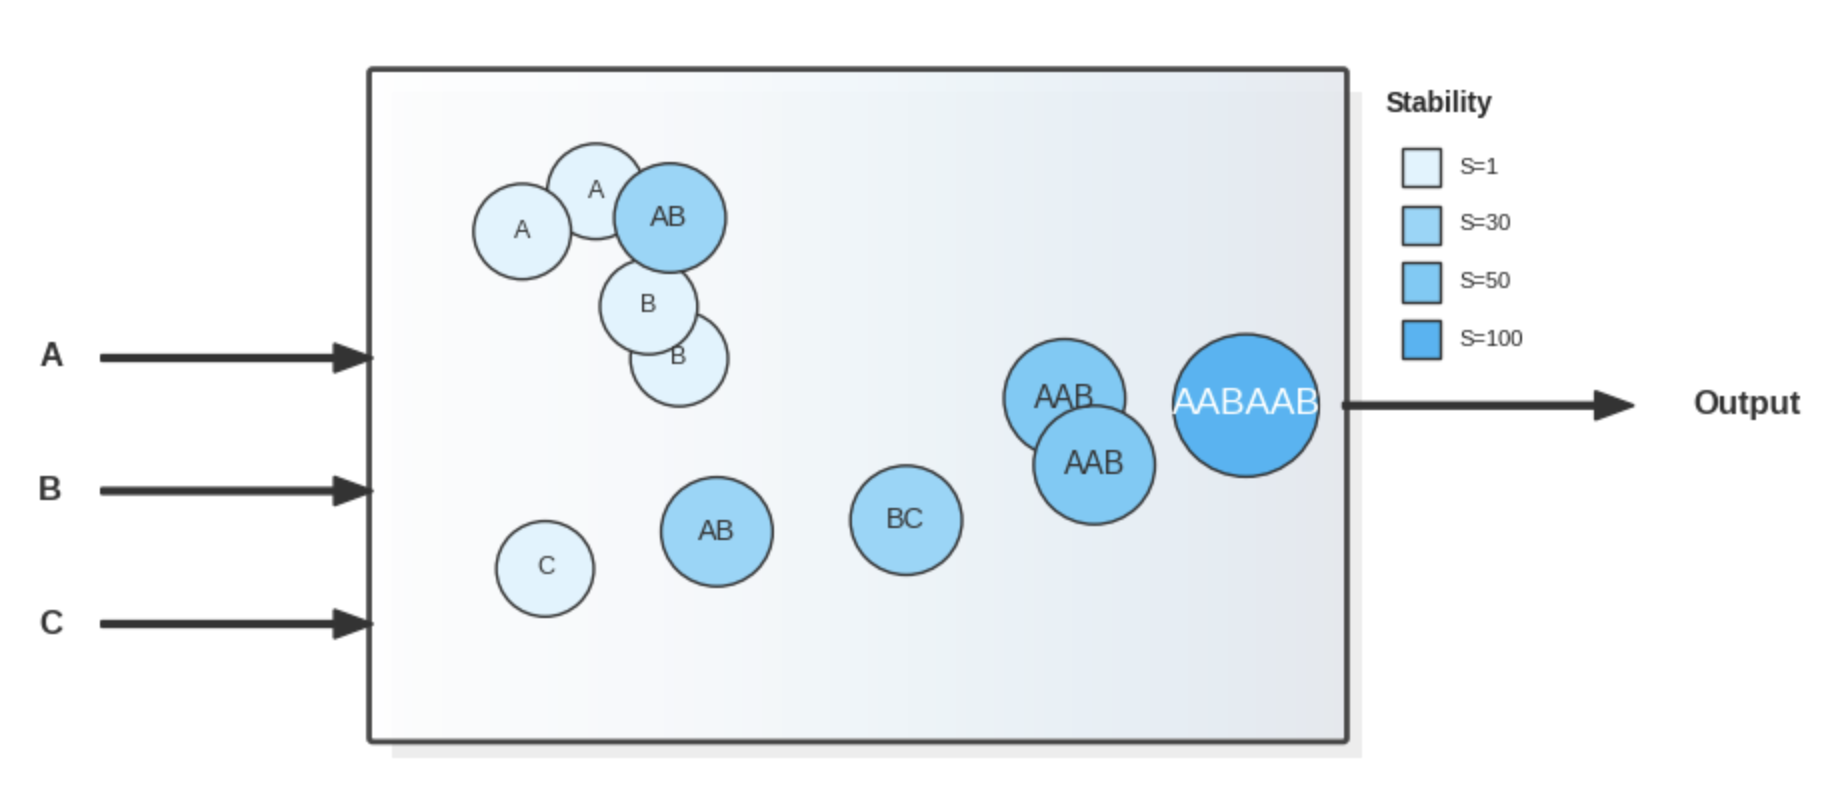
\includegraphics[width=0.9\textwidth]{figure_1}
    \caption{SDA analogue of a chemical Continuous Flow Stirred Tank Reactor (CFSTR)}
    \label{fig:figure_1}
\end{figure}

\subsection{Formal Definition}

A Stability-Driven Assembly (SDA) system is formally defined as a tuple $(E, P, S, R, I)$ where:
\begin{itemize}
   \item $E = \{e_1, e_2, \ldots, e_n\}$ is a finite set of base elements
   \item $P$ is the set of all possible patterns formed by concatenating elements from $E$ and existing patterns
   \item $S: P \rightarrow \mathbb{Z}^{+}$ is a stability function mapping each pattern to a non-negative integer representing its lifetime
   \item $R: E \rightarrow \mathbb{Z}^{+}$ is a replenishment function specifying how many copies of each base element are added per generation
   \item $I \in \mathbb{Z}^{+}$ is the number of interactions allowed per generation
\end{itemize}

The pattern interaction operation, denoted by $\oplus$, is defined as a string concatenation. When patterns $p_1$ and $p_2$ interact, they form a pattern $p_1 \oplus p_2$.

\begin{algorithm}[H]
\caption{SDA System Simulation}
\footnotesize
\begin{algorithmic}[1]
\REQUIRE Base elements $E$, stability function $S$, replenishment rates $R$, interaction count $I$, generations $T$
\ENSURE Pattern population evolution over $T$ generations
\STATE Initialize population with base elements
\FOR{$t = 1$ to $T$}
   \STATE Remove expired patterns
   \STATE Add $R(e)$ copies of each element $e \in E$ to population
   \FOR{$i = 1$ to $I$}
       \STATE Select patterns $p_1$, $p_2$ randomly from population
       \STATE Form $p_{new} = p_1 \oplus p_2$
       \STATE Set expiration time for $p_{new}$ to $t + S(p_{new})$
       \STATE Add $p_{new}$ to population
   \ENDFOR
\ENDFOR
\end{algorithmic}
\end{algorithm}

The probability of selecting a pattern $p$ for interaction is proportional to its frequency in the population. This creates a feedback mechanism: patterns with higher stability persist longer, becoming more abundant, which increases their probability of participating in interactions.

\subsection{Illustrative Example}

Consider a simple SDA system with base elements \( A \) and \( B \), where \( AB \) has a lifetime of 10 generations, \( ABAB \) has a lifetime of 50 generations, and all other compounds degrade instantly. After the first generation, only \( A \), \( B \), and \( AB \) persist due to the instantaneous degradation of unstable patterns such as \( AA \) and \( BB \). As \( AB \) persists due to its longer life, its abundance naturally increases, increasing the probability of forming \( ABAB \). This dynamic reflects a form of roulette wheel selection \cite{goldberg1989genetic, holland1975adaptation}, where stability-driven persistence affects interaction probability. The emergent pattern \( ABAB \) represents a higher-order configuration, demonstrating how selection shapes evolutionary pathways through differential stability.

\begin{figure}[htp]
    \centering
    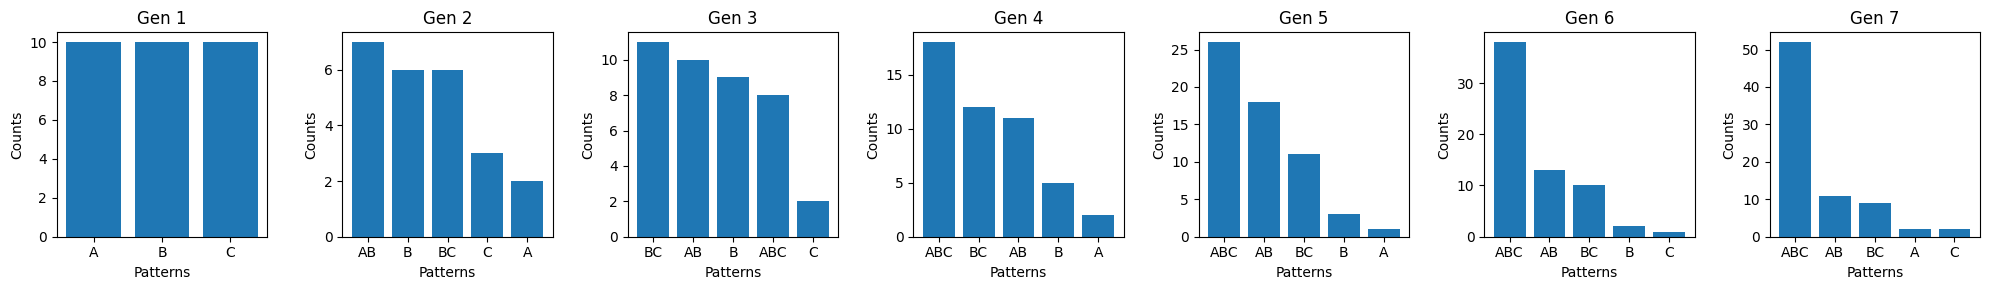
\includegraphics[width=1\textwidth]{figure_2}
    \caption{SDA System population evolution simulation}
    \label{fig:figure_2}
\end{figure}

The apparent entropy reduction in Figure \ref{fig:figure_2} occurs without a Maxwell demon \cite{leff2002maxwell}. Compounds that persist longer have more chances to interact, and as their frequency increases, their interaction probability grows further. This fitness-proportionate selection mechanism \cite{back1996evolutionary, goldberg1989genetic, holland1975adaptation} drives the system to lower-entropy states.

\section{Probabilistic Dynamics and Entropy Evolution in SDA Systems}

SDA systems can be analyzed through probabilistic models that explain how stability-driven selection shapes population dynamics and entropy evolution.

\subsection{Population and Stability Distributions}

Two key distributions characterize SDA systems: the \textbf{population distribution} representing the abundance of the pattern, defined as \( P_t(p) = \frac{N_t(p)}{\sum_{q \in P} N_t(q)} \), where \( N_t(p) \) is the count of the pattern \( p \) at generation \( t \); and the \textbf{stability function} \( S: P \rightarrow \mathbb{Z}^{+} \) mapping each pattern to its lifetime. In real-world applications, the stability values would be determined by domain-specific principles such as binding energies, activation barriers, or competitive advantages.

\subsection{Pattern Evolution Model}

The probability of observing pattern \(p\) in generation \(t+1\) is the result of two processes: persistence of existing copies and creation of new copies through interactions. For persistence analysis, we account for pattern instances with different creation times:
\begin{equation}
\label{eq:persist-term}
\mathrm{Persist}_t(p) = P_t(p) \cdot \left(1 - \frac{1}{\overline{R}_t(p)}\right)
\end{equation}

Here \(\overline{R}_t(p)\) represents the average remaining lifetime of the pattern instances \(p\) at generation \(t\). In a system with constant creation rates, \(\overline{R}_t(p)\) would approach \(\frac{S(p)+1}{2}\). For creation analysis, we estimate the probability of forming new copies through concatenations:
\begin{equation}
\label{eq:create-term}
\mathrm{Create}_t(p) = \sum_{(q,r) \to p} P_t(q) \cdot P_t(r)
\end{equation}

Here, \((q,r) \to p\) indicates pattern pairs that form pattern \(p\) when concatenated. The combined population distribution at the next generation is:
\begin{equation}
\label{eq:full-ba-update}
P_{t+1}(p) = \frac{
  \mathrm{Persist}_t(p) + \mathrm{Create}_t(p)
}{
  \sum_{p' \in P} 
  \left[
    \mathrm{Persist}_t(p') + \mathrm{Create}_t(p')
  \right]
}
\end{equation}

\subsection{Entropy Dynamics}

The expected entropy change between generations can be expressed as:
\begin{equation}
\Delta H = H(P_{t+1}) - H(P_t)
\end{equation}

The relative influence of persistence versus creation is quantified by parameter $\alpha$:
\begin{equation}
\alpha = \frac{\sum_p \mathrm{Persist}_t(p)}{\sum_p \mathrm{Persist}_t(p) + \sum_p \mathrm{Create}_t(p)}
\end{equation}

When $\alpha$ approaches 1, stability-driven selection dominates; when it approaches 0, random creation processes predominate. The entropy change can be approximated as:
\begin{equation}
\Delta H \approx (1 - \alpha) \cdot \Delta H_{create} + \alpha \cdot \Delta H_{persist}
\end{equation}

Where $\Delta H_{create}$ represents the change in entropy from creation processes (typically positive) and $\Delta H_{persist}$ represents the change in entropy from stability-driven persistence (typically negative). These two competing dynamics may cause the entropy to oscillate.

\subsection{Simulation Results}

Our simulations comparing SDA systems to unconstrained systems confirm that SDA systems consistently maintain a lower entropy due to stability-driven selection (Figure~\ref{fig:figure_3}).

\begin{figure}[h]
    \centering
    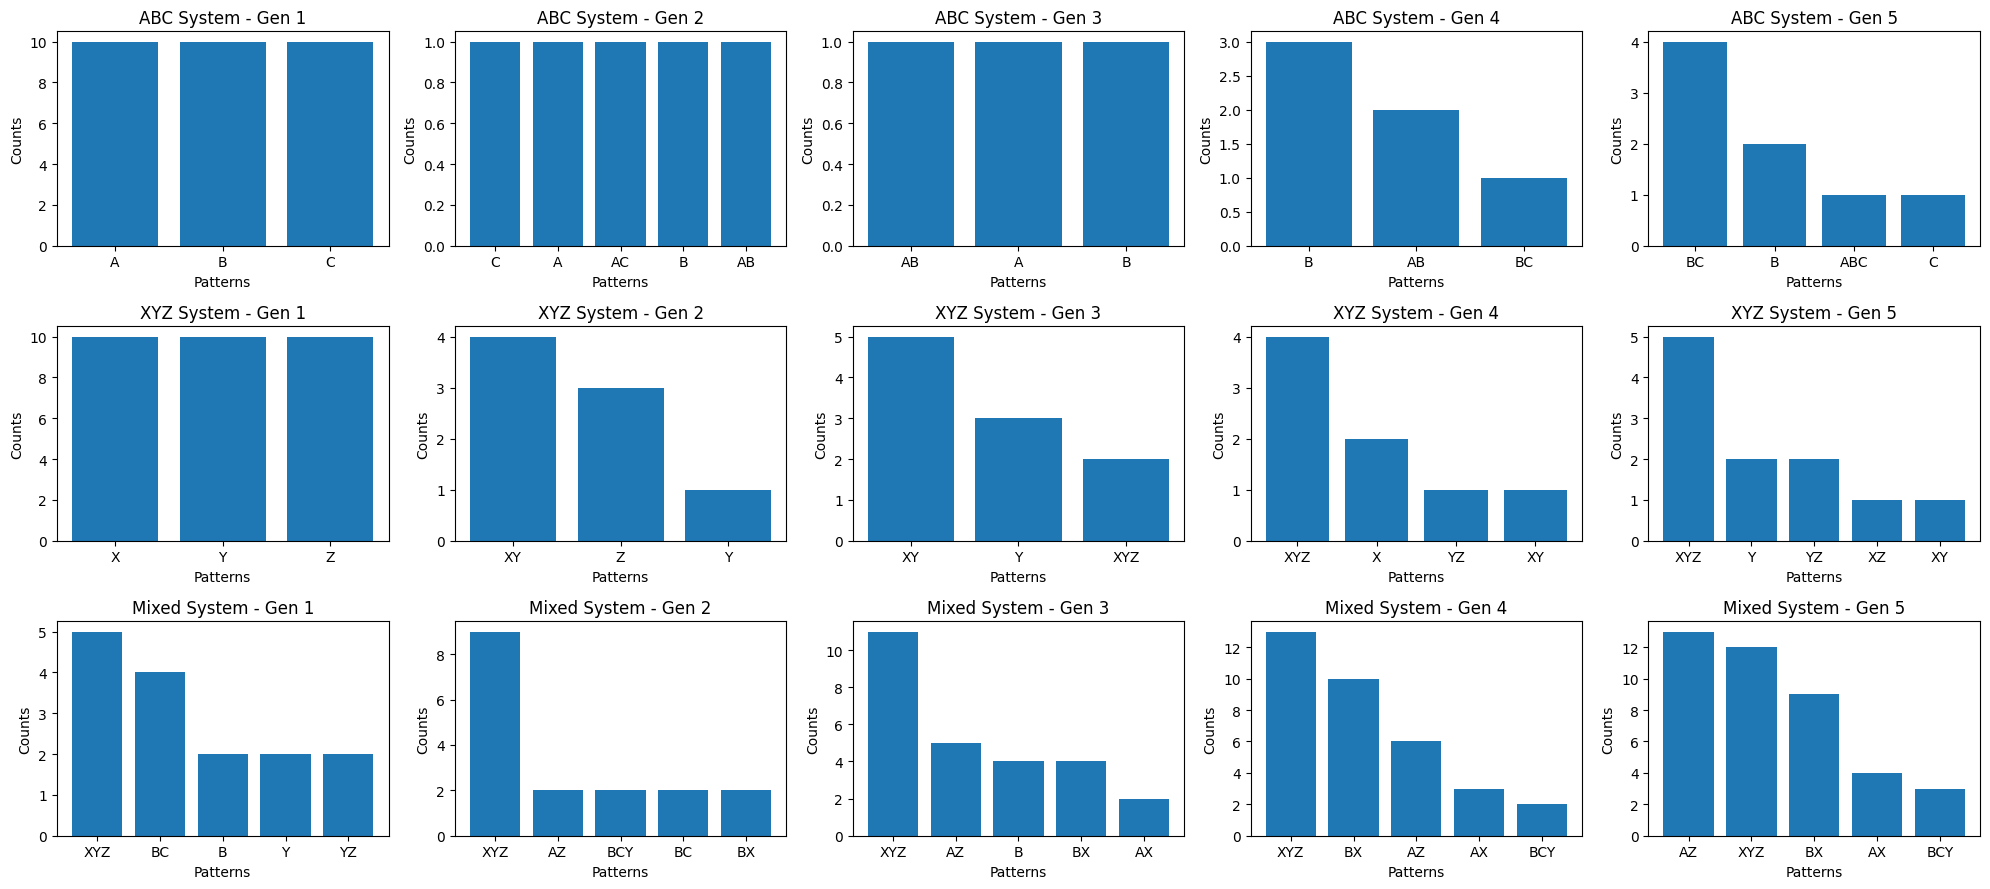
\includegraphics[width=0.7\textwidth]{figure_3.png}
    \caption{The SDA system consistently maintains lower entropy due to selection.}
    \label{fig:figure_3}
\end{figure}

SDA systems exhibit significantly different pattern distributions, with high-stability patterns dominating the population (Figure~\ref{fig:figure_4}).

\begin{figure}[h]
    \centering
    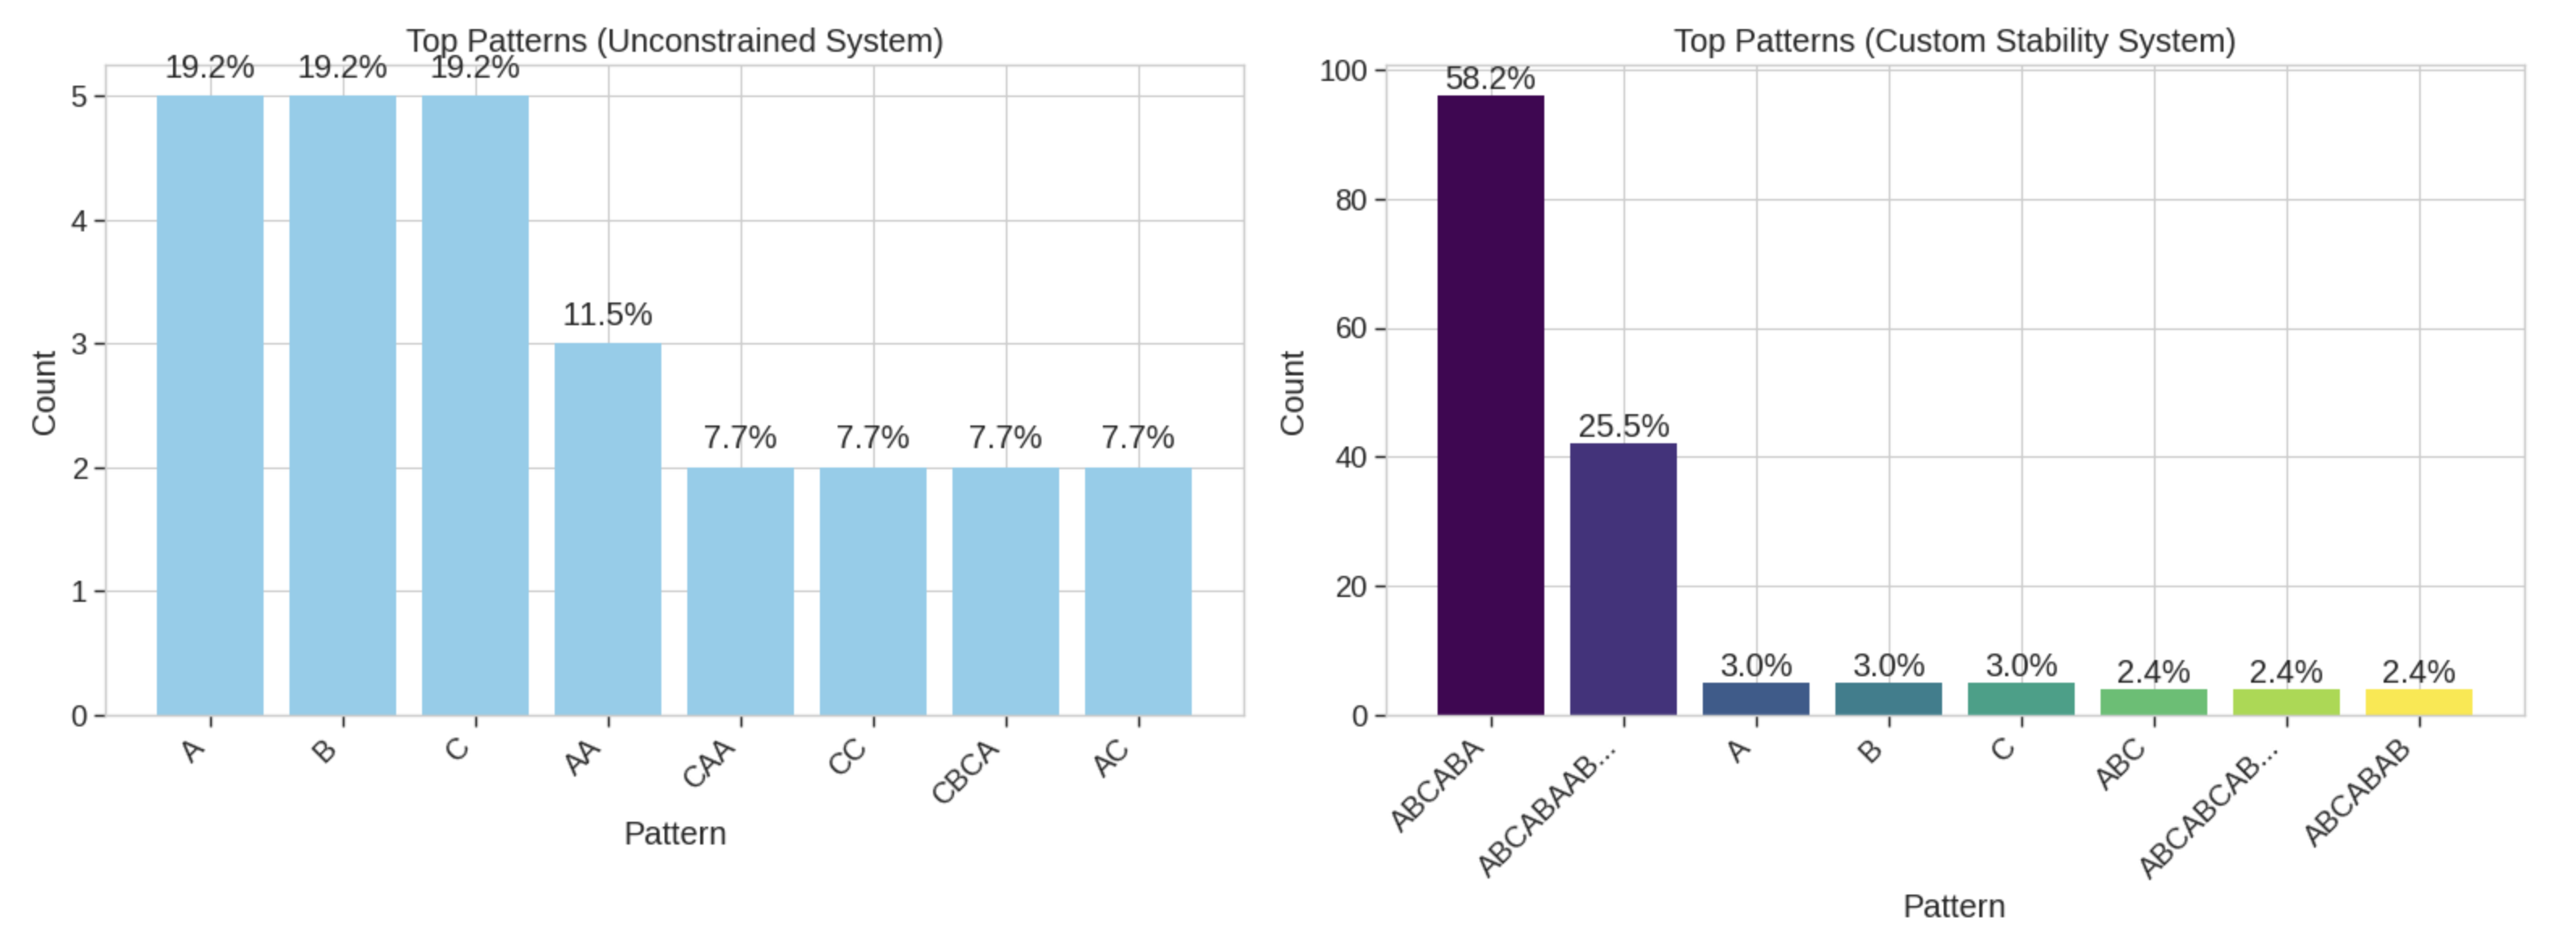
\includegraphics[width=0.9\textwidth]{figure_4}
    \caption{The SDA system (right) shows dominance of stable patterns, while the unconstrained system (left) exhibits a more uniform distribution.}
    \label{fig:figure_4}
\end{figure}

Interestingly, SDA systems with multiple high-stability patterns often exhibit oscillatory behavior in entropy over time (Figure~\ref{fig:figure_5}).

\begin{figure}[h]
    \centering
    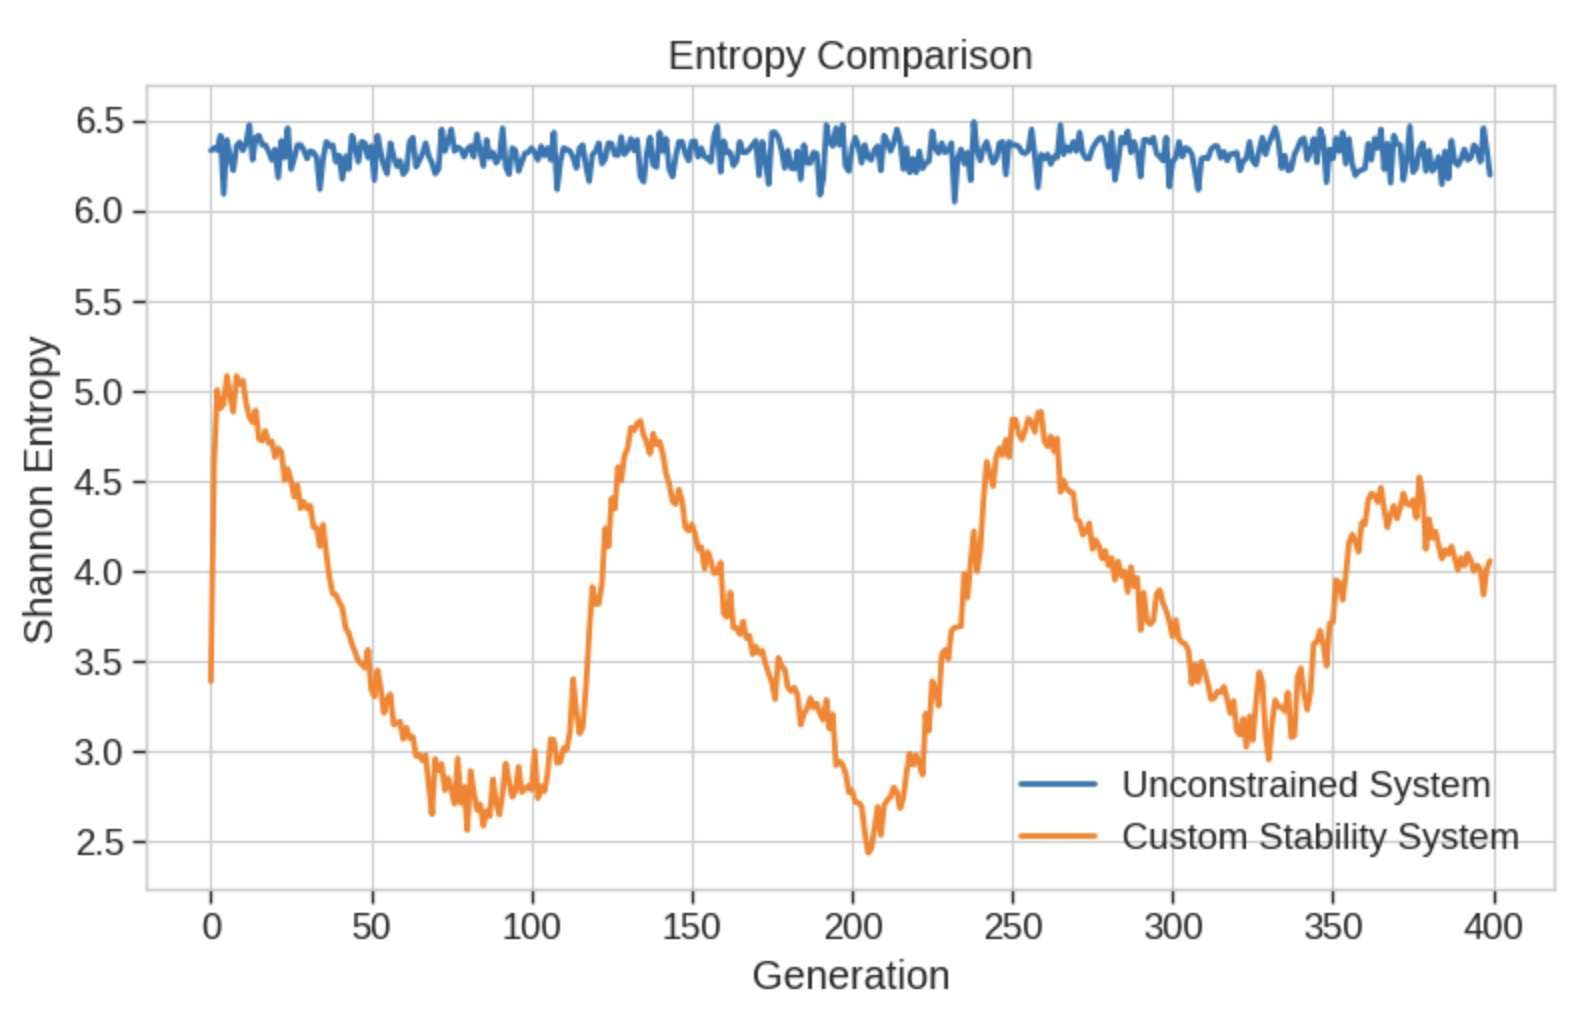
\includegraphics[width=0.7\textwidth]{figure_5}
    \caption{Oscillatory entropy dynamics in an SDA system.}
    \label{fig:figure_5}
\end{figure}

\subsection{Dynamical Systems Interpretation}

The oscillatory behavior resembles the coupled oscillator networks analyzed by Strogatz \cite{strogatz2001exploring}. Adapting this framework to SDA systems, oscillation periods can be approximated by:

\begin{equation}
T \approx \beta \sqrt{\frac{I \cdot S_1 \cdot S_2}{|S_1 - S_2|}}
\end{equation}

Where $I$ is the interaction rate, $S_1$ and $S_2$ are the stabilities of the dominant patterns, and $\beta$ is a system-specific constant. These oscillations demonstrate that SDA systems exhibit rich dynamics driven by the interplay between pattern formation and stability-driven selection, allowing exploration of different pattern-space regions while maintaining entropy lower than that of unconstrained systems.



\section{Intervention Analysis of Stability-Driven Assembly Systems}

To test the causal relationship between stability constraints and system evolution, we conducted controlled intervention experiments that systematically altered stability parameters mid-simulation, allowing us to isolate the direct impact of stability on pattern distribution and entropy.

\subsection{Experimental Design}

We implemented two key intervention experiments:

\begin{enumerate}
    \item \textbf{Unconstrained to SDA}: System with uniform stability values for 400 generations, then stability constraints are introduced.
    
    \item \textbf{SDA to Unconstrained}: System with differential stability for 400 generations, then all constraints are removed.
\end{enumerate}

For both experiments, we maintained identical parameters for the replenishment of the base element (rate = 5) and the frequency of interaction (100 interactions per generation). The stability function assigned significantly higher values to certain patterns:

\begin{equation}
S(p) = 
\begin{cases}
100, & \text{if } p = \text{ABCABA} \\
50, & \text{if } p \in \{\text{ABA, ABC}\} \\
30, & \text{if } p \in \{\text{AB, BC}\} \\
1, & \text{otherwise}
\end{cases}
\end{equation}

\subsection{Unconstrained to SDA Transition}

When transitioning from an unconstrained regime to a stability-driven regime, we observed pronounced changes in system behavior. Figure~\ref{fig:u2s-entropy} shows the evolution of the entropy at this transition point.

\begin{figure}[h]
    \centering
    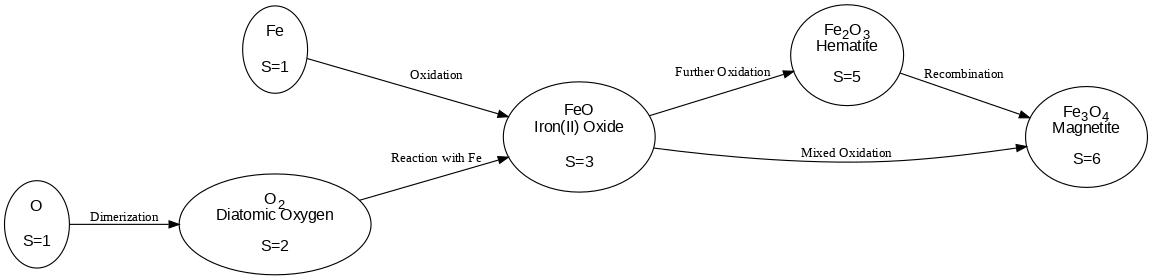
\includegraphics[width=0.6\textwidth]{figure_6.png}
    \caption{Entropy evolution when transitioning from Unconstrained $\to$ SDA system. The vertical dashed line marks the intervention point.}
    \label{fig:u2s-entropy}
\end{figure}


\begin{figure}[h]
    \centering
    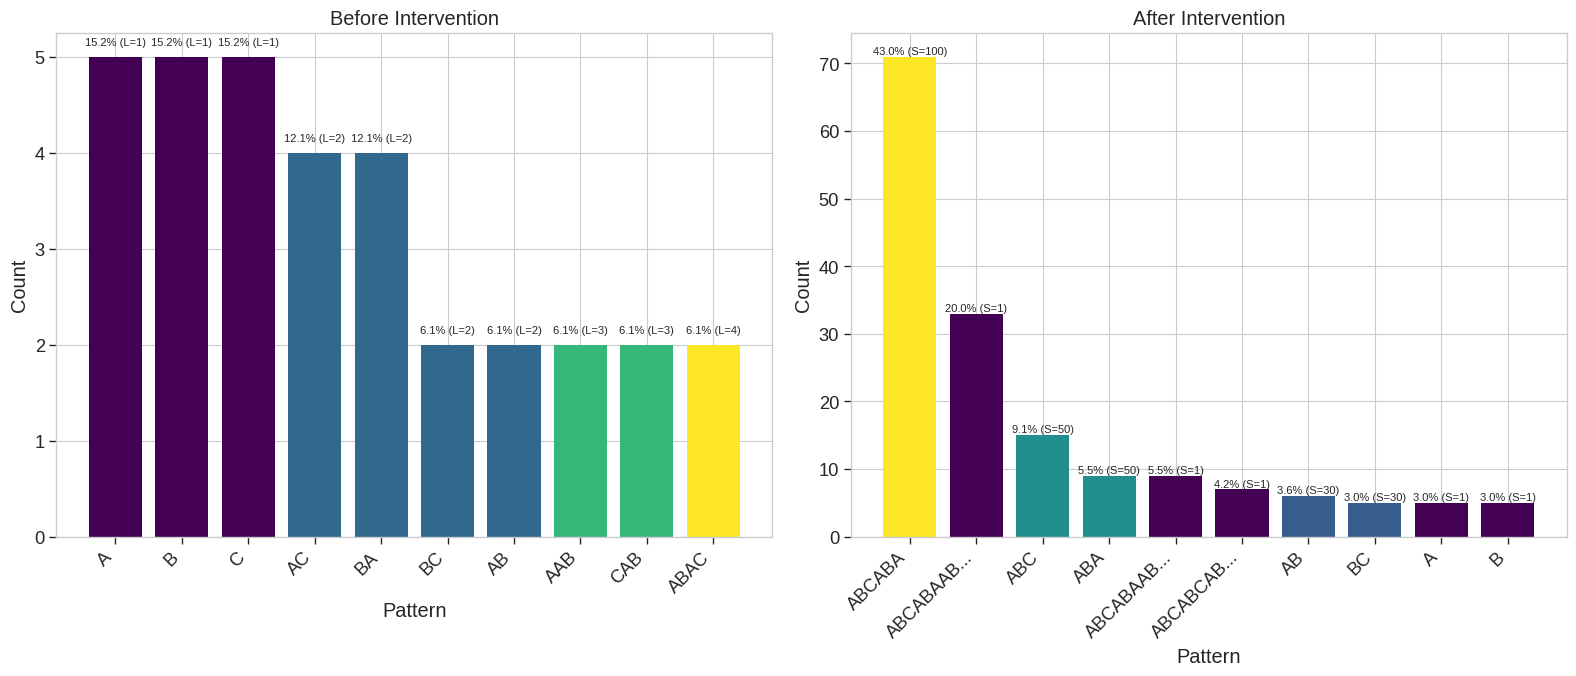
\includegraphics[width=0.6\textwidth]{figure_7.png}
    \caption{Pattern composition before (left) and after (right) transitioning from an unconstrained to an SDA system. Bar colors represent stability values.}
    \label{fig:u2s-patterns}
\end{figure}

Before intervention, the system exhibited the high entropy characteristic of an unconstrained regime. After imposing the stability function at generation 400, the entropy decreased rapidly before settling into oscillations. Figure~\ref{fig:u2s-patterns} reveals the pattern composition before and after the intervention.

In the unconstrained phase, the pattern distribution remained relatively uniform. After introducing stability constraints, the system evolved toward dominance by patterns with higher assigned stability values, supporting the prediction that stability acts as a selective force.

\subsection{SDA to Unconstrained Transition}

To establish bidirectional causality, we examined the transition from a stability-driven regime to an unconstrained regime. Figure~\ref{fig:s2u-entropy} shows the evolution of the entropy during this reverse intervention, and Figure~\ref{fig:s2u-patterns} shows how pattern distribution becomes more random.

\begin{figure}[h]
    \centering
    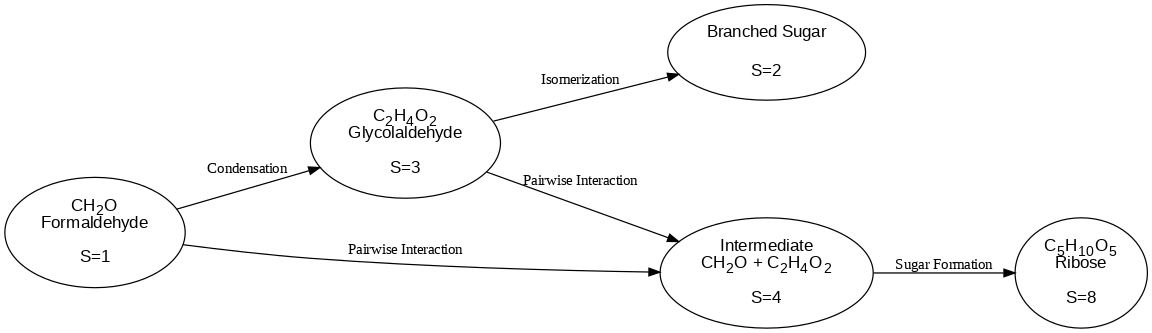
\includegraphics[width=0.6\textwidth]{figure_8.png}
    \caption{Entropy evolution when transitioning from an SDA $\to$ an unconstrained system.}
    \label{fig:s2u-entropy}
\end{figure}

\begin{figure}[h]
    \centering
    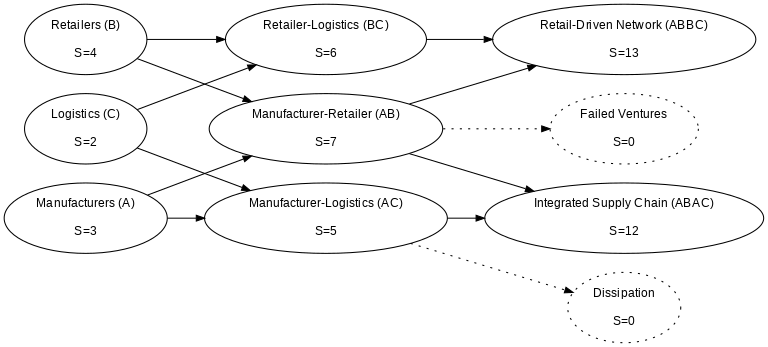
\includegraphics[width=0.6\textwidth]{figure_9.png}
    \caption{Pattern composition before (left) and after (right) transitioning from an SDA to an unconstrained system. Bar colors represent stability values.}
    \label{fig:s2u-patterns}
\end{figure}

Before intervention, the SDA system oscillated around low entropy values of ~4 bits. Upon removal of stability constraints at generation 400, entropy increased within 100 generations as stable patterns died out, and the system returned to a more uniform distribution with entropy over 6 bits.

\subsection{Causal Inference and Evolutionary Dynamics}

The symmetrical and opposite responses to intervention in both experiments provide strong evidence of causality. When stability constraints are imposed, the entropy decreases; when it is removed, the entropy increases. This symmetry suggests that stability acts as a control parameter directly determining the system's entropy state.

These dynamics align with the principles of fitness-weighted selection in evolutionary systems, where persistence and reproductive opportunity drive the emergence of dominant patterns. SDA systems exhibit genuine evolutionary behavior arising from differential persistence through two reinforcing mechanisms.
\begin{enumerate}
    \item \textbf{Persistence advantage}: Higher-stability patterns accumulate more copies over time.
    \item \textbf{Frequency-dependent selection}: As patterns become more frequent, they participate in proportionally more interactions.
\end{enumerate}

These findings establish that stability-driven selection can account for the emergence of ordered, nonrandom pattern distributions without requiring explicit replication mechanisms. By preferentially preserving certain configurations based solely on their persistence properties, SDA systems provide a minimal framework for understanding how complexity and information can accumulate in systems far from equilibrium.


\section{Bidirectional Causation in SDA Systems}

SDA systems exhibit a distinctive interplay between bottom-up and top-down causal influences, creating feedback loops that drive complexity emergence.

\begin{figure}[h]
    \centering
    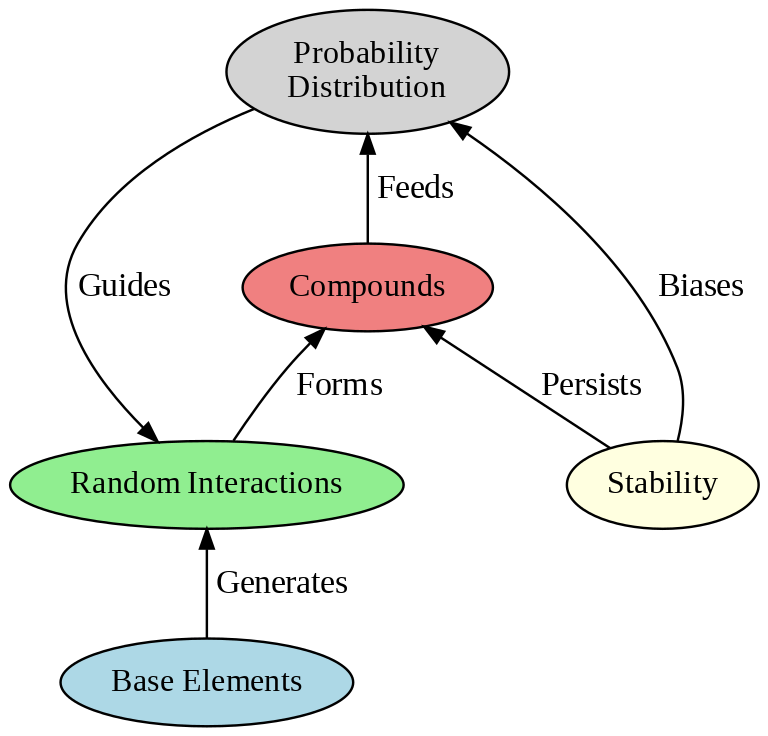
\includegraphics[width=0.7\linewidth,height=0.7\linewidth]{figure_10.png}
    \caption{Bottom-up and Top-down causation in SDA systems}
    \label{fig:figure_10}
\end{figure}

As shown in Figure~\ref{fig:figure_10}, bottom-up processes arise from the probabilistic assembly of base elements into increasingly complex patterns. Simultaneously, top-down influence emerges as stable patterns accumulate, increasing their relative abundance, and directing subsequent interactions. This bidirectional causation creates a self-reinforcing dynamic where emergent structures shape future interactions.

This mechanism distinguishes SDA systems from traditional statistical mechanics \cite{landau1980statistical}, where macrostates represent aggregate properties but do not directly influence microstate interaction rules. In SDA systems, dominant patterns exert causal influence on micro-level interactions, embedding history and specificity into the generative process itself. As patterns persist on the basis of stability, they statistically bias the system toward interactions that involve them, creating a form of feedback that drives pattern evolution.

Such explicit interplay suggests a broader principle: emergent structures can become causal agents that direct further system evolution. This perspective helps explain the accumulation of novel order in contexts ranging from prebiotic chemistry to computational networks, where higher-level assemblies increasingly govern local interactions, catalyzing the exploration of new possibilities.

At times, these dynamics appear teleological, as if the system were "seeking" more stable configurations. However, as Bertalanffy \cite{bertalanffy1968general} noted, such processes reflect the natural unfolding of selection and feedback loops rather than purposeful design. SDA systems illustrate how feedback from emergent structures can drive the exploration of new system states without implying predetermined goals, providing a model for complexity accumulation through iterative processes of selection and the continual reshaping of local interactions.

\section{Network Representation and Applications of SDA Systems}

\subsection{Dynamic Network Representation}

\begin{figure}[h]
    \centering
    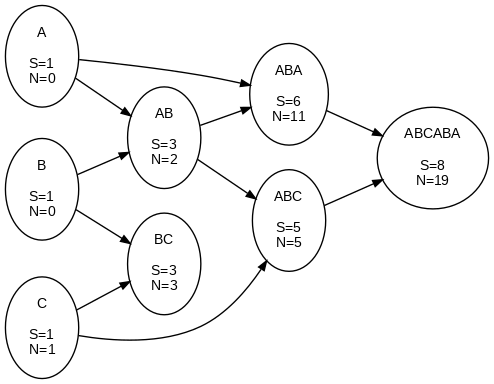
\includegraphics[width=0.4\linewidth]{figure_11.png}
    \caption{Early generation of SDA network with patterns ABA and ABC dominating.}
    \label{fig:figure_11}
\end{figure}

SDA systems can be visualized as directed networks, where nodes represent patterns (base elements and compounds), and edges represent assembly interactions. This network perspective reveals how stability shapes pattern evolution through token flow dynamics.

\begin{figure}[h]
    \centering
    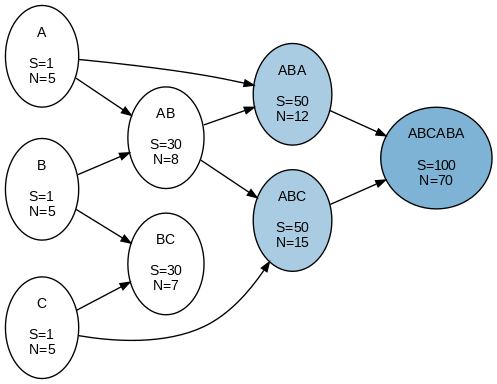
\includegraphics[width=0.5\linewidth]{figure_12.png}
    \caption{Later generation of SDA network with pattern ABCABA dominating.}
    \label{fig:figure_12}
\end{figure}

As shown in Figure~\ref{fig:figure_11} Figure~\ref{fig:figure_12}, tokens (representing pattern instances) accumulate at nodes based on stability values, creating preferential flow paths through the network. Nodes with higher stability (\textit{e.g.}, $ABCABA$) attract more tokens, leading to self-reinforcing dominance. This phenomenon parallels physical systems where high-conductivity channels divert flow from existing pathways, similar to the dynamics observed in fluid systems and RC circuits.

The network structure may undergo significant reorganization if a "disruptor node" with high stability emerges, rerouting token flows, and redistributing resources. Importantly, this network representation reveals common descent relationships between patterns, where child patterns inherit structural elements from their parent patterns, reflecting a fundamental feature of evolution: branching lineages of descent with modification. This phylogenetic aspect of the network allows researchers to trace the evolutionary history of complex patterns back to their simpler ancestors. The overall dynamic resembles switch-level simulation of transistor networks \cite{AdlerCAD}, where network pathways are determined by the state of activated transistors, which guides the current flow.

\subsection{\added{Forward Kolmogorov Perspective on SDA}}

\added{The network representation of SDA can be understood through the Forward Kolmogorov (master equation) formalism, which governs how probability mass flows among discrete states over time:}

\begin{equation}
\label{eq:kolmogorov-general}
\frac{dP_t(p)}{dt}
= \sum_{q} W_{q \to p}(t) P_t(q)
- \sum_{r} W_{p \to r}(t) P_t(p),
\end{equation}

\added{where $W_{q \to p}(t)$ and $W_{p \to r}(t)$ are inflow and outflow rates for pattern node $p$. In conventional master equation models (e.g., MAK models in the Appendix), these rates are fixed externally. In SDA, in contrast, flows are biased by fixed stability values assigned to patterns. Relative stability differences between patterns skew the probability distribution, so that over time, more stable patterns gain weight while less stable ones lose it. As the population distribution evolves, the effective flow rates change with it, producing a recursive distribution-dependent drift field unique to the SDA model.}

\added{This recursive dependence makes it natural to describe SDA systems as \emph{evolving}. In the Kolmogorov framework, probability continuously flows between patterns, biased by their relative stability. Because the drift is shaped by the current distribution, the system explores, selects, and retains structures over time rather than settling into equilibrium. Entropy change in SDA thus reflects an evolutionary process in which stability acts as a selection principle shaping system trajectories. A fuller connection to non-linear Fokker–Planck dynamics will be developed in future work.}




\subsection{Application Examples}



\subsubsection{Chemical Example: Iron Oxidation}

\begin{figure}[h]
    \centering
    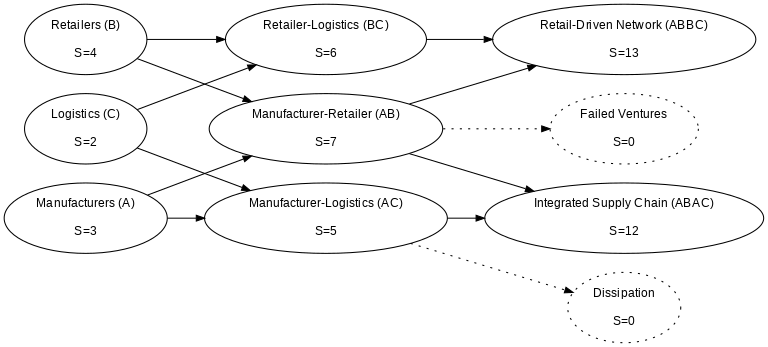
\includegraphics[width=1\textwidth,height=0.3\textwidth]{figure_13.png}
    \caption{Reaction network for iron oxidation, illustrating the formation of stable and intermediate compounds under stability constraints.}
    \label{fig:figure_13}
\end{figure}

Figure~\ref{fig:figure_13} illustrates iron oxidation as an SDA system, where oxygen (\(O_2\)) reacts with iron to produce increasingly stable oxides, including iron(II) oxide (\(FeO\)), iron(III) oxide (\(Fe_2O_3\), hematite, and iron (II,III) oxide (\(Fe_3O_4\), magnetite). The stability values (\(S(p)\)) quantify the persistence of each compound, with higher values assigned to products with robust bonding and lower susceptibility to dissociation. This reaction network demonstrates how stability shapes chemical pathways, favoring reactions that lead to more persistent products.

\added{This example is provided as an \emph{illustrative heuristic} rather than a chemically parameterized kinetics model. Reversibility and detailed kinetic rates are not modeled here. The purpose is to show how SDA captures the directional bias imposed by relative stability: less stable intermediates lose probability weight to more persistent oxides, exemplifying how stability-driven flows favor durable structures.}


\subsubsection{Economic Example: Industry Ecosystem}

\begin{figure}[h]
    \centering
    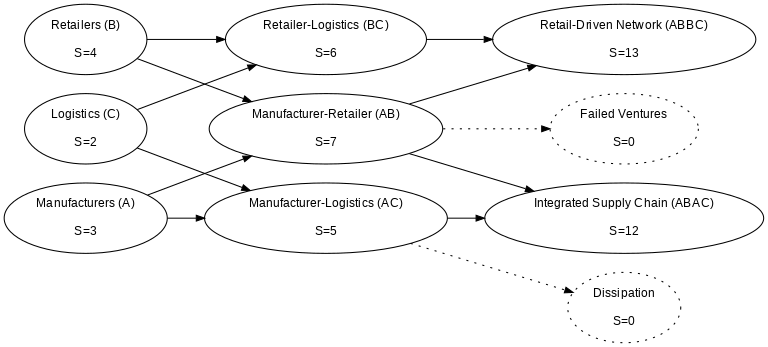
\includegraphics[width=1\textwidth]{figure_14.png}
    \caption{Industry ecosystem represented as an SDA system, showing evolution from base businesses to integrated networks.}
    \label{fig:figure_14}
\end{figure}

Figure~\ref{fig:figure_14} models an economic ecosystem in which manufacturers (A), retailers (B), and logistics providers (C) form increasingly more complex partnerships and integrated networks. Stable configurations such as manufacturer-retailer partnerships (\( AB \)) and retail-driven networks (\( ABBC \)) act as attractors, accumulating resources over time. Less viable business configurations dissipate quickly, redistributing resources to more stable arrangements.

These examples demonstrate how the SDA framework provides a unifying perspective on pattern formation across diverse domains. In each case, stability serves as the key driver of selection, guiding system evolution without requiring explicit replication mechanisms.

\subsection{Natural Manifestations of Stability-Driven Selection}

SDA systems abstract principles observable across diverse natural processes where differential persistence creates selection pressure without explicit replication. Crystal formation demonstrates how molecular configurations with lower energy states persist longer, driving systems towards ordered structures \cite{ball1999self}. Similarly, sand dune patterns emerge from the differential stability of formations under specific wind conditions, while river networks evolve as more efficient drainage pathways persist and less stable configurations are reconfigured during flood events \cite{kelso1997dynamic}.

These natural manifestations share a key property with SDA systems: apparent directionality toward complexity through nothing more than persistence differentials and probabilistic interactions. The framework enables testable predictions about pattern formation in physical and chemical systems. For example, SDA predicts plateau-like transitions in complexity metrics - periods of stasis followed by rapid shifts as new stable patterns emerge, aligned with complexity measurement approaches such as integrated information theory \cite{tononi2008phi}.

Additionally, SDA systems predict pseudo-homochirality emergence under certain stability constraints. When one stereoisomer achieves greater stability than its mirror image, differential persistence should drive the system toward domination by the more stable configuration \cite{blackmond2010chiral}. Laboratory experiments could test how stability differentials alone might contribute to symmetry breaking in prebiotic chemical systems.

By abstracting away specific physical mechanisms to focus on stability-driven selection, the SDA framework bridges the conceptual gap between inanimate physical processes guided by energetic principles and the evolutionary dynamics characteristic of biological systems.

\section{Conclusion}

Stability-Driven Assembly (SDA) systems provide a rigorous framework for understanding the emergence of complexity in systems governed by probabilistic interactions and stability-driven selection. Our computational experiments and mathematical analysis demonstrate that differential stability alone can generate selection pressure, driving systems toward lower-entropy states dominated by stable patterns.

Our intervention experiments conclusively established causality between stability constraints and system evolution. When transitioning between unconstrained and stability-driven regimes, entropy changes predictably and reversibly, confirming that stability functions as a control parameter shaping the evolutionary landscape. These findings substantiate the possibility that selection can emerge spontaneously from stability differences without explicit replication mechanisms.

The dynamic network representation revealed how high-stability nodes naturally accumulate resources, establishing preferential pathways that reinforce their dominance across generations. This perspective bridges micro-level interactions with macro-level pattern distributions, showing how local stability differences translate into global order.

The interplay between bottom-up and top-down causation illuminates how persistent patterns exert increasing influence on subsequent interactions, creating feedback loops that amplify their representation. This recursive dynamic distinguishes SDA systems from frameworks where higher-level states merely describe, rather than causally influence, lower-level processes.

Applications to diverse domains, from chemical reactions to economic networks, demonstrate the broad explanatory power of the SDA framework. In each case, stability-driven selection provides a unifying mechanism for understanding how order emerges from probabilistic interactions.

These findings suggest that evolution may be a more universal property than previously recognized, potentially operating in any system with large stability imbalances. By demonstrating how random populations naturally evolve toward order through stability-driven interactions, this framework proposes that biological evolution may represent a specialized instance of a more general phenomenon.

Future work may focus on experimental validation in physical systems, mathematical models with energetic constraints, and the interaction of stability-driven selection with other evolutionary mechanisms. Additionally, developing dynamical models to map system responses across various regions of the hyperparameter space of patterns would provide a more comprehensive understanding of stability-driven selection's scope and limitations. The framework's application should also extend beyond its current domains to diverse fields including physics (e.g. self-organizing quantum systems), biochemistry (metabolic network evolution), geology (mineral formation pathways), atmospheric sciences (persistent weather patterns), materials science (self-assembly of nanostructures), and information theory (emergence of computational primitives), where differential stability may be driving emergent complexity.

%\begin{listing}[H]
%\caption{Title of the listing}
%\rule{\columnwidth}{1pt}
%\raggedright Text of the listing. In font size footnotesize, small, or normalsize. Preferred format: left aligned and single spaced. Preferred border format: top border line and bottom border line.
%\rule{\columnwidth}{1pt}
%\end{listing}

%%%%%%%%%%%%%%%%%%%%%%%%%%%%%%%%%%%%%%%%%%
\vspace{6pt} 

%%%%%%%%%%%%%%%%%%%%%%%%%%%%%%%%%%%%%%%%%%
%% optional
%\supplementary{The following supporting information can be downloaded at:  \linksupplementary{s1}, Figure S1: title; Table S1: title; Video S1: title.}

% Only for journal Methods and Protocols:
% If you wish to submit a video article, please do so with any other supplementary material.
% \supplementary{The following supporting information can be downloaded at: \linksupplementary{s1}, Figure S1: title; Table S1: title; Video S1: title. A supporting video article is available at doi: link.}

% Only for journal Hardware:
% If you wish to submit a video article, please do so with any other supplementary material.
% \supplementary{The following supporting information can be downloaded at: \linksupplementary{s1}, Figure S1: title; Table S1: title; Video S1: title.\vspace{6pt}\\
%\begin{tabularx}{\textwidth}{lll}
%\toprule
%\textbf{Name} & \textbf{Type} & \textbf{Description} \\
%\midrule
%S1 & Python script (.py) & Script of python source code used in XX \\
%S2 & Text (.txt) & Script of modelling code used to make Figure X \\
%S3 & Text (.txt) & Raw data from experiment X \\
%S4 & Video (.mp4) & Video demonstrating the hardware in use \\
%... & ... & ... \\
%\bottomrule
%\end{tabularx}
%}

%%%%%%%%%%%%%%%%%%%%%%%%%%%%%%%%%%%%%%%%%%

%\funding{This research received no external funding}

%\institutionalreview{Not applicable}

%\informedconsent{Not applicable}

%\dataavailability{Not applicable} 

%\acknowledgments{}

%\conflictsofinterest{The author declares no conflicts of interest} 

%%%%%%%%%%%%%%%%%%%%%%%%%%%%%%%%%%%%%%%%%%
%%%%%%%%%%%%%%%%%%%%%%%%%%%%%%%%%%%%%%%%%%
%%%%%%%%%%%%%%%%%%%%%%%%%%%%%%%%%%%%%%%%%%
%\printendnotes[custom] % Un-comment to print a list of endnotes

% Please provide either the correct journal abbreviation (e.g. according to the “List of Title Word Abbreviations” http://www.issn.org/services/online-services/access-to-the-ltwa/) or the full name of the journal.
% Citations and References in Supplementary files are permitted provided that they also appear in the reference list here. 

%=====================================
% References, variant A: external bibliography
%=====================================
%\bibliography{your_external_BibTeX_file}

%=====================================
% References, variant B: internal bibliography
%=====================================
\begin{thebibliography}{999}

\bibitem{kauffman1995home}
Kauffman, S. \textit{At Home in the Universe: The Search for the Laws of Self-Organization and Complexity}; Oxford University Press: New York, NY, USA, 1995.

\bibitem{fisher1930genetical}
Fisher, R.A. \textit{The Genetical Theory of Natural Selection}; Oxford University Press: Oxford, UK, 1930.

\bibitem{davies2006goldilocks}
Davies, P. \textit{The Goldilocks Enigma: Why is the Universe Just Right for Life?}; Allen Lane: London, UK, 2006.

\bibitem{hordijk2012autocatalytic}
Hordijk, W.; Steel, M.; Kauffman, S. The structure of autocatalytic sets: Evolvability, enablement, and emergence. \textit{Acta Biotheoretica} \textbf{2012}, \textit{60}, 379–392.

\bibitem{nghe2015prebiotic}
Nghe, P.; Hordijk, W.; Kauffman, S.A.; Walker, S.I.; Schmidt, F.J.; Kemble, H.; Yeates, J.A.; Lehman, N. Prebiotic network evolution: Six key parameters. \textit{Molecular BioSystems} \textbf{2015}, \textit{11}, 3206–3217.

\bibitem{kolmogorov1965complexity}
Kolmogorov, A.N. Three Approaches to the Quantitative Definition of Information. \textit{Problemy Peredachi Informatsii} \textbf{1965}, \textit{1}, 3–11.

\bibitem{chaitin1977algorithmic}
Chaitin, G.J. Algorithmic Information Theory. \textit{IBM J. Res. Dev.} \textbf{1977}, \textit{21}, 350–359.

\bibitem{solomonoff1964formal}
Solomonoff, R.J. A Formal Theory of Inductive Inference. Part I and Part II. \textit{Inf. Control} \textbf{1964}, \textit{7}, 1–22, 224–254.

\bibitem{shannon1948mathematical}
Shannon, C.E. A Mathematical Theory of Communication. \textit{Bell Syst. Tech. J.} \textbf{1948}, \textit{27}, 379–423.

\bibitem{deutsch2013constructor}
Deutsch, D.; Marletto, C. Constructor theory of information. \textit{Proceedings of the Royal Society A: Mathematical, Physical and Engineering Sciences} \textbf{2015}, \textit{471}, 20140540.

\bibitem{walker2023nature}
Walker, S.I.; Cronin, L.; et al. Assembly theory explains and quantifies selection and evolution across physical and biological systems. \textit{Nature} \textbf{2023}, \textit{618}, 619-628.

\bibitem{schrodinger1944life}
Schrödinger, E. \textit{What is Life?}; Cambridge University Press: Cambridge, UK, 1944.

\bibitem{pross2016life}
Pross, A. \textit{What is Life? How Chemistry Becomes Biology}; Oxford University Press: Oxford, UK, 2016.

\bibitem{kauffman1986autocatalytic}
Kauffman, S.A. Autocatalytic sets of proteins. \textit{Journal of Theoretical Biology} \textbf{1986}, \textit{119}, 1–24.

\bibitem{hordijk2011required}
Hordijk, W.; Kauffman, S.A.; Steel, M. Required levels of catalysis for emergence of autocatalytic sets in models of chemical reaction systems. \textit{International Journal of Molecular Sciences} \textbf{2011}, \textit{12}, 3085–3101.

\bibitem{fontana1991algorithmic}
Fontana, W. Algorithmic chemistry. \textit{Artificial Life II} \textbf{1991}, \textit{11}, 159–209.

\bibitem{barabasi1999emergence}
Barabási, A.-L.; Albert, R. Emergence of scaling in random networks. \textit{Science} \textbf{1999}, \textit{286}, 509–512.

\bibitem{nowak2006evolutionary}
Nowak, M.A. \textit{Evolutionary Dynamics: Exploring the Equations of Life}; Belknap Press: Cambridge, MA, USA, 2006.

\bibitem{england2015dissipative}
England, J.L. Dissipative adaptation in driven self-assembly. \textit{Nature Nanotechnology} \textbf{2015}, \textit{10}, 919–923.

\bibitem{wu2012origin}
Wu, M.; Higgs, P.G. Origin of self-replicating biopolymers: Autocatalytic feedback can trump power law replication. \textit{Journal of Molecular Evolution} \textbf{2012}, \textit{74}, 91–102.

\bibitem{prigogine1977self}
Prigogine, I.; Nicolis, G. \textit{Self-Organization in Non-Equilibrium Systems}; Wiley: New York, NY, USA, 1977.

\bibitem{nicolis1977self}
Nicolis, G.; Prigogine, I. \textit{Self-Organization in Nonequilibrium Systems: From Dissipative Structures to Order through Fluctuations}; Wiley: New York, NY, USA, 1977.

\bibitem{noble2012causality}
Noble, D. A Theory of Biological Relativity: No Privileged Level of Causation. \textit{Interface Focus} \textbf{2012}, \textit{2}, 55–64.

\bibitem{ellis2012top}
Ellis, G.F.R. Top-down causation and emergence: Some comments on mechanisms. \textit{Interface Focus} \textbf{2012}, \textit{2}, 126–140.

\bibitem{lloyd2006programming}
Lloyd, S. \textit{Programming the Universe: A Quantum Computer Scientist Takes on the Cosmos}; Alfred A. Knopf: New York, NY, USA, 2006.

\bibitem{wolfram2020fundamental}
Wolfram, S. \textit{A Project to Find the Fundamental Theory of Physics}; Wolfram Media: Champaign, IL, USA, 2020.

\bibitem{ball1999self}
Ball, P. \textit{The Self-Made Tapestry: Pattern Formation in Nature}; Oxford University Press: New York, NY, USA, 1999.

\bibitem{kelso1997dynamic}
Kelso, J.A.S. \textit{Dynamic Patterns: The Self-Organization of Brain and Behavior}; MIT Press: Cambridge, MA, USA, 1997.

\bibitem{blackmond2010chiral}
Blackmond, D.G. The origin of biological homochirality. \textit{Cold Spring Harbor Perspectives in Biology} \textbf{2010}, \textit{2}, a002147.

\bibitem{tononi2008phi}
Tononi, G. Consciousness as Integrated Information: A Provisional Manifesto. \textit{Biological Bulletin} \textbf{2008}, \textit{215}, 216–242.

\bibitem{fogler1999chemical}
Fogler, H.S. \textit{Elements of Chemical Reaction Engineering} (3rd ed.). Prentice Hall, 1999.

\bibitem{petri1962communication}
Petri, C.A. Communication with Automata. Technical Report RADC-TR-65-377, Rome Air Development Center, New York, 1966.

\bibitem{goldberg1989genetic}
Goldberg, D.E. \textit{Genetic Algorithms in Search, Optimization, and Machine Learning}; Addison-Wesley: Boston, MA, USA, 1989.

\bibitem{holland1975adaptation}
Holland, J.H. \textit{Adaptation in Natural and Artificial Systems}; University of Michigan Press: Ann Arbor, MI, USA, 1975.

\bibitem{back1996evolutionary}
Bäck, T.; Fogel, D.B.; Michalewicz, Z. \textit{Evolutionary Computation 1: Basic Algorithms and Operators}; CRC Press: FL, USA, 2000.

\bibitem{leff2002maxwell}
Leff, H.S.; Rex, A.F. \textit{Maxwell's Demon: Entropy, Information, Computing}; Princeton University Press: Princeton, NJ, USA, 2002.

\bibitem{strogatz2001exploring}
Strogatz, S.H. Exploring complex networks. \textit{Nature} \textbf{2001}, \textit{410}, 268–276.

\bibitem{landau1980statistical}
Landau, L.D.; Lifshitz, E.M. \textit{Statistical Physics}; Pergamon Press, 1980.

\bibitem{bertalanffy1968general}
Bertalanffy, L. von. \textit{General System Theory}; George Braziller: New York, NY, USA, 1968.

\bibitem{AdlerCAD}
Adler, D. Switch Level Simulation Using Dynamic Graph Algorithms. \textit{IEEE Transactions on Computer-Aided Design of Integrated Circuits and Systems} \textbf{1991}, \textit{10}.

\bibitem{TuranyiTomlin2014}
Turányi, T.; Tomlin, A.S. \textit{Analysis of Kinetic Reaction Mechanisms}; Springer: Berlin, Germany, 2014.

\bibitem{heylighen2019chemical}
Heylighen, F.; Beigi, S.; Veloz, T. Chemical Organization Theory as a modeling framework for self-organization, autopoiesis and resilience. International Journal of General Systems, \textbf{2019}, \textit{48}(7), 682-705.

\end{thebibliography}

%% Add \usepackage{lineno} before \begin{document} and uncomment 
%% following line to enable line numbers
%% \linenumbers

\appendix

\section{Mass Action Kinetics and SDA Systems}

Mass Action Kinetics (MAK) \cite{TuranyiTomlin2014} provides deterministic rate equations for chemical reactions:
\[
\frac{d[A]}{dt} = -k [A][B]
\]
where $[A]$ and $[B]$ represent concentrations and $k$ is a rate constant. Chemical Organization Theory (COT) \cite{heylighen2019chemical} emphasizes closed self-maintained collections of species in fixed reaction networks, while Assembly Theory (AT) uses MAK-like models to link object production to assembly indices.

Although MAK excels at describing known reactions under equilibrium assumptions, it inherently models bidirectional reactions with fixed rates within predefined networks, unlike SDA which emphasizes net forward construction and allows open discovery of novel compounds.

\subsection{Analogy to Electronic Circuit Simulations}

MAK models represent the evolution of species concentration as $\dot{\mathbf{x}} = \mathbf{A}\mathbf{x} + \mathbf{b}$, where \(\mathbf{x}\) represents concentrations, \(\mathbf{A}\) encodes rate constants, and \(\mathbf{b}\) accounts for replenishment. This parallels electronic circuit simulation, where the node voltages evolve as $\dot{\mathbf{v}} = \mathbf{A}\mathbf{v} + \mathbf{b}$.

Higher-level circuit abstractions, such as switch-level simulation \cite{AdlerCAD}, track discrete state transitions rather than solving full ODEs, while gate-level models treat circuits as idealized logical operations. Similarly, SDA systems capture dominant generational updates rather than modeling bidirectional flows explicitly. This abstraction, analogous to switch-level circuit simulation , allows SDA to focus on net forward assembly steps that determine pattern persistence and evolution.


\section{Stability Imbalances in Nature}

The SDA model is motivated by natural stability disparities, from fleeting nuclear states to enduring gravitational structures. These variations in binding energy and system resilience dictate the formation of low-entropy structures across scales. The persistence of structures is influenced by multiple factors, including spatial arrangements, catalytic reinforcement, and hierarchical assembly.

\begin{table}
\centering
\caption{Representative Stability Mechanisms in Nature and Their Typical Lifetimes.}
\label{tab:binding-forces}
\footnotesize
\begin{tabular}{l l}
\toprule
\textbf{Mechanism} & \textbf{Typical Lifetime} \\
\midrule
Weak Nuclear (Beta Decay) & $\mu$s to minutes \\
Strong Nuclear (Stable Nuclei) & Millions to trillions of years \\
Covalent Bonds & Seconds to billions of years \\
Hydrogen Bonding & Picoseconds to seconds \\
Ionic Bonds & Seconds to millennia \\
Geological Structures & Thousands to billions of years \\
Gravitational Systems & Millions to billions of years \\
\bottomrule
\end{tabular}
\end{table}

This hierarchy of stability mechanisms, spanning twenty orders of magnitude in persistence times, illustrates how stability-driven selection shapes the emergence of low-entropy structures across nature. From quantum-level interactions to cosmic architecture, differential persistence creates an implicit selection pressure without requiring explicit replication machinery. The universal presence of these stability gradients suggests that selection may be more fundamental than previously recognized: a core property of physical reality rather than a specialized biological phenomenon.

When viewed through the lens of SDA theory, natural systems can be seen as engaged in a process of information accumulation through stability-driven pattern persistence. The patterns emerging from these systems—whether molecular configurations, geological formations, or galactic structures—represent a form of encoded memory about their environments and interaction histories. This perspective establishes a conceptual bridge between physical self-organization and biological evolution.

By formalizing stability-driven selection in the SDA framework, we provide a mathematical foundation for understanding how complexity and information emerge from simple physical processes.


\end{document}

\endinput
%%
%% End of file `elsarticle-template-num.tex'.
